\documentclass[10pt,pdf,hyperref={unicode}]{beamer}
\usepackage{verbatim}

\setbeamertemplate{blocks}[rounded=true, shadow=true]
\setbeamertemplate{footline}[page number]
\usepackage{multicol}

\usefonttheme{serif}
\beamertemplatenavigationsymbolsempty

\usepackage[utf8]{inputenc}
\usepackage[english, russian]{babel}
\usepackage{amsmath,mathrsfs,mathtext}
\usepackage{graphicx, epsfig}
\usepackage{caption}
\usepackage{subfig}
\usepackage{amsmath, bm}
\usepackage{algorithm}

\usepackage{algorithmic}

\usepackage{tabularx}

\usepackage{tikz}

\DeclareMathOperator*{\argmin}{arg\,min}
\DeclareMathOperator*{\argmax}{arg\,max}

\makeatletter
\let\@@magyar@captionfix\relax
\makeatother

\usetheme{Warsaw}
\usecolortheme{sidebartab}
\definecolor{beamer@blendedblue}{RGB}{31,49,120}

\setbeamertemplate{enumerate items}[circle]

\setbeamersize{text margin left=1.5em, text margin right=1.5em}

\usepackage{ragged2e}

%----------------------------------------------------------------------------------------------------------
\title[\hbox to 56mm{Определение сложности выборки \hfill\insertframenumber\,/\,\inserttotalframenumber}]
{Определение сложности выборки с помощью универсальной аппроксимирующей модели}
\author[Малиновский Г. С.]{\Large Малиновский Григорий Станиславович}
\institute{ Московский физико-технический институт\\
Факультет управления и прикладной математики\\
Кафедра интеллектуальных систем\\

}

\date{\footnotesize{\emph{ММРО - 2019, }г. Москва }}
%----------------------------------------------------------------------------------------------------------
\begin{document}
%----------------------------------------------------------------------------------------------------------
\begin{frame}
\titlepage
\end{frame}

\begin{frame}{Постановка задачи}
\justifying
\textbf{Цель:} предложить способ построения набора моделей локальной аппроксимации для решения задач классификации и регрессии.

~\\
\textbf{Задачи}

\begin{enumerate}
	\justifying
	\item Проверка адекватности выборки для обобщенно-линейной модели
	\item Оптимизировать структурные параметры выбираемых моделей по порождающей выборке с целью получения выборки с оптимальными свойствами.

\end{enumerate}

~\\
\textbf{Исследуемая проблема}
	\justifying
	~\\
	Исследование свойств промежуточного параметрического пространства, строящегося моделями локальной аппроксимации. 
	
~\\
\textbf{Методы решения}
\justifying
~\\
Применение параметров униварсальной аппроксимирующей модели для определения сложности выборки





\end{frame}

\begin{frame}{Список литературы}
\begin{itemize}
	\justifying
	\item \textit{A.M. Katrutsa, V.V. Strijov} Stress test procedure for feature selection algorithms~// Chemometrics and Intelligent Laboratory Systems 142, 172-183.
	
	\item \textit{A.A. Aduenko, A.P. Motrenko, V.V. Strijov} Object selection in credit scoring using covariance matrix of parameters estimations~// Annals of Operations Research, 2018, 260(1-2) : 3-21.
	
	\item	\textit{G.V. Cybenko} Approximation by Superpositions of a Sigmoidal function~// Mathematics of Control Signals and Systems. -- 1989. -- Т. 2, № 4. -- С. 303--314.
	
	\item \textit{L. Ling, Y.S. Abu-Mostafa} Data complexity in machine learning~// Computer Science Technical Reports, 2006.003.
	
	\item \textit{A.C.~Lorena, A.I.~Maciel, P.B.C.~de~Miranda, I.G.~Costa, R.B.C.~Prudencio} Data complexity meta-features for regression problems~// Machine Learning 107 (1), 209-246
	
	
\end{itemize}
\end{frame}

\begin{frame}{Постановка задачи}
\justifying
\textbf{Задан временной ряд}
	$$S: T \rightarrow \mathbb{R}, \text{где } T = \left\lbrace t_0, t_0+d, t_0+2d, \ldots\right\rbrace $$.
\textbf{Определен сегмент временного ряда}
	$$\mathbf{x}_{i}=\left[S\left(t_{i}\right), S\left(t_{i}-d\right), S\left(t_{i}-2 d\right), \ldots, S\left(t_{i}-(n-1) d\right)\right]^{\top}, \quad \mathbf{x}_{i} \in X \equiv \mathbb{R}^{n}$$
\textbf{Задана выборка}\\
$\mathfrak{D}=\left\{\left(\mathbf{x}_{i}, y_{i}\right)\right\}_{i=1}^{l}, \quad y_{i} \in\{1,2, \ldots K\}.$\\
$\mathbf{X} \in \mathbb{X}$ --- множество наборов сегментов временного ряда.\\
$\mathbf{Y} \in \mathbb{Y}$ --- множество меток классов движения (бег, ходьба, подъем) в случае задачи классификации;  исследуемая величина (температура тела, давление) в случае задачи регрессии. \\
\textbf{Требуется найти отображение}
$$f:\mathbb{X} \rightarrow \mathbb{Y}, \text{ где } \mathbb{Y} = \{1,2, \ldots K\} \text{ или } \mathbb{R} $$
\end{frame}
\begin{frame}{Локальная аппроксимация}
\justifying
\textbf{Модель локальной аппроксимации}
$$g_i(\mathbf{w},\mathbf{x})\in \mathbb{X}, \text{ где } w \in \mathbb{W} = \mathbb{R}^{n_g}$$
Оптимальные параметры находятся из решения задачи 
$$\mathbf{w}^{opt}_i = \arg \min _{\mathbf{w} \in \mathbb{R}^{n_{\mathbf{g}}}} \rho(g_i(\mathbf{w}, \mathbf{x}), \mathbf{x}), \text{ где } \rho \text{ --- функция расстояния}$$
\textbf{Промежуточное пространство}\\
Данная процедура задает отображение из пространства сегментов временных рядов в пространство параметров.
$$ h:\mathbb{X} \rightarrow \mathbb{Z} \subseteq \mathbb{W} $$
Пространство $\mathbb{Z}$ будем называть промежуточным пространством признаковых описаний.




\end{frame}

\begin{frame}{Схема построения алгоритма}
\justifying
\textbf{Общая схема}\\
\begin{center}
	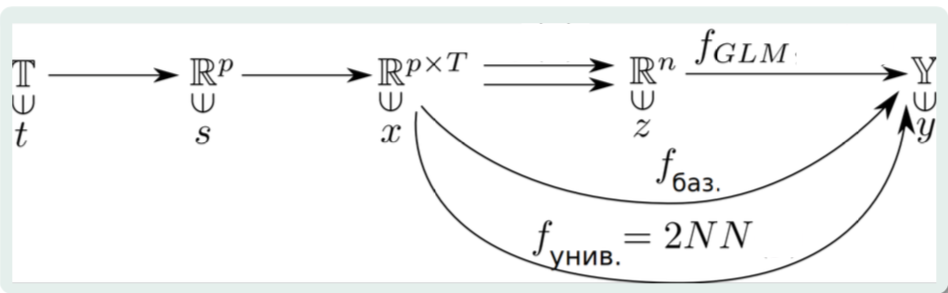
\includegraphics[width=1\textwidth]{scheme.png}
\end{center}
$$\mathbb{X}\xrightarrow{f_{\text{баз}}(\mathbf{x})}\mathbb{Y} =  \mathbb{X}\xrightarrow{h(\mathbf{x})}\mathbb{Z}\xrightarrow{f_{GLM}(\mathbf{z})}\mathbb{Y}$$
Требуется проанализировать, может ли выборка промежуточного признакового описания быть адекватно описана обобщенно-линейной моделью.


\end{frame}

\begin{frame}{Коэффициенты детерминации}
	\justifying
	\small
\begin{block}{Определение 1}
	\textbf{Коэффициент детерминации $R^2$}\\
	В случае задачи регрессии будем определять коэффициент по формуле:
	$$R^{2}=1-\frac{\sum_{i=1}^{N}\left(y_{i}-\hat{y}_{i}\right)^{2}}{\sum_{i=1}^{N}\left(y_{i}-\bar{y}\right)^{2}}$$
	где $y_i$ --- истинные ответы, $\hat{y}_i$ --- предсказания модели, $\bar{y}$ --- среднее значение.
\end{block}





\begin{block}{Определение 2}
		\justifying
		\small
	\textbf{Коэффициент детерминации pseudo-$R^2$}\\
	В случае классификации будем определять коэффициент по формуле:
	$$R^{2}=1-\frac{\ln \hat{L}\left(M \right)}{\ln \hat{L}\left(M_{\text {Null}}\right)}$$\\
	где $\hat{L}\left(M \right)$ --- правдоподобие исследуемой модели, $\hat{L}\left(M_{\text {Null}}\right)$ --- правдоподобие константной модели.
\end{block}
\end{frame}
\begin{frame}{Универсальная модель}
\justifying
\small
Рассмотрим двухслойную полносвязную нейронную сеть.
\begin{center}
	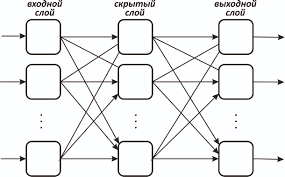
\includegraphics[width=0.4\textwidth]{2NN.png}
\end{center}
\begin{block}{Теорема Цыбенко}
	\justifying
	Пусть $\varphi$ любая непрерывная сигмоидная функция, например, $\varphi(\xi) = 1/(1 + e^{-\xi})$. Тогда, если дана любая непрерывная функция действительных переменных $f$ на $[0, 1]^n$ (или любое другое компактное подмножество $\mathbb{R}^n$) и $\varepsilon > 0$, то существуют векторы $\mathbf{w_1}, \mathbf{w_2}, \dots, \mathbf{w_N}, \mathbf{\alpha}$ и $\mathbf{\theta}$ и параметризованная функция $G(\mathbf{\cdot}, \mathbf{w}, \mathbf{\alpha}, \mathbf{\theta}): [0, 1]^n \to \mathbb{R}$ такая, что для всех $\mathbf{x} \in [0,1]^n$ выполняется
	: $\big|G(\mathbf{x}, \mathbf{w}, \mathbf{\alpha}, \mathbf{\theta}) - f(\mathbf{x})\big| < \varepsilon,$
	где
	: $G(\mathbf{x}, \mathbf{w}, \mathbf{\alpha}, \mathbf{\theta}) = \sum_{i=1}^N \alpha_i \varphi(\mathbf{w}_i^T \mathbf{x} + \theta_i),$
	и $\mathbf{w}_i \in \mathbb{R}^n,$ $\alpha_i, \theta_i \in \mathbb{R},$ $\mathbf{w} = (\mathbf{w}_1, \mathbf{w}_2, \dots, \mathbf{w}_N),$ $\mathbf{\alpha} = (\alpha_1, \alpha_2, \dots, \alpha_N),$ и $\mathbf{\theta} = (\theta_1, \theta_2, \dots, \theta_N).$
\end{block}

\end{frame}

\begin{frame}{Определение сложности}
\begin{block}{Определение 3}
	\justifying
	\textbf{Сложностью универсальной модели} будем называть количество нейронов $n_{uni}$ на скрытом слое 
\end{block}
\begin{block}{Определение 4}
	\justifying
	\textbf{Сложностью переобучения для выборки} будем называть минимальное число нейронов на скрытом слое универсальной модели, при котором коэффициент детерминации равен 1.
	$$ comp_{fit}(\mathfrak{D}) = \argmin_{n_{uni}\in \mathbb{N}} n_{uni}| R^2(\mathfrak{D},n_{uni}) = 1$$
\end{block}
\begin{block}{Следствие 1}
	\justifying 
	Для любой возможной выборки сложность переобучения меньше бесконечности.\\
	Доказательство следует из определения и теоремы Цыбенко.
\end{block}
\end{frame}
\begin{frame}{Мультиколлинеарный анализ}
\justifying
Пусть задана выборка
$$\mathfrak{D}=\left\{\left(\mathbf{x}_{i}, y_{i}\right)\right\}_{i=1}^{m} = \{(\mathbf{X}, \mathbf{y})\}$$

Представим нашу выборку в виде:
$$ \mathbf{X}=\left[X_{1}, \ldots, X_{j}, \ldots, X_{n}\right], \mathbf{X} \in \mathbb{R}^{m \times n} \text { and } j \in \mathcal{J}=\{1, \ldots, n\}$$
$$\mathbf{y} = [y_1,\ldots,y_m] \in \mathbb{Y}\subset \mathbb{R}^m$$
Полагаем, что все признаки и вектор ответов нормализованы
$$\|\mathbf{y}\|_{2}=1 \text { and }\left\|x_{j}\right\|_{2}=1, j \in \mathcal{J}$$
Далее введем определения мультиколлинеарности и скоррелированности 
\end{frame}
\begin{frame}{Мультиколлинеарность и скоррелированность}
\begin{block}{Определение 5}
	\justifying
	\small
	Признаки с индексами из множества $A$ мультиколлениарны, если существует индекс $j$, коэффициенты $a_k$ и множество индексов $\{k\}\subset A\setminus j$,  существует достаточно малое число $\delta>0$	---  степень мультиколлинеарности, такое что
	$$\left\|x_{j}-\sum_{k=A\setminus j} a_{k} x_{k}\right\|_{2}^{2}<\delta$$

\end{block}
\begin{block}{Определение 6}
	\justifying
	\small
	Признаки с индексами $i,j$ скоррелированны, если существует достаточно малое число $\delta_{i,j}>0$, такое что
	$$\left\|x_{i}-x_{j}\right\|_{2}^{2}<\delta_{i,j}$$
\end{block}
\begin{block}{Определение 7}
	\justifying
	\small
	Признак с индексом $j$ скоррелирован с вектором ответов, если существует   существует достаточно малое число $\delta>0$, такое что
	$$\left\|\mathbf{y}-x_{j}\right\|_{2}^{2}<\delta_{y j}$$
\end{block}
\end{frame}

\begin{frame}{Конфигурации данных}
\begin{figure}[H]
	\begin{minipage}[h]{0.47\linewidth}
		\center{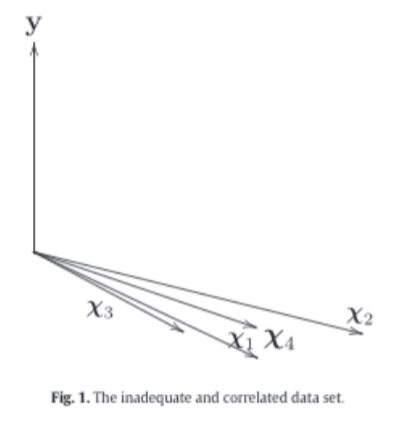
\includegraphics[width=.7\linewidth]{q2.png}}  \\
	\end{minipage}
	\hfill
	\begin{minipage}[h]{0.47\linewidth}
		\center{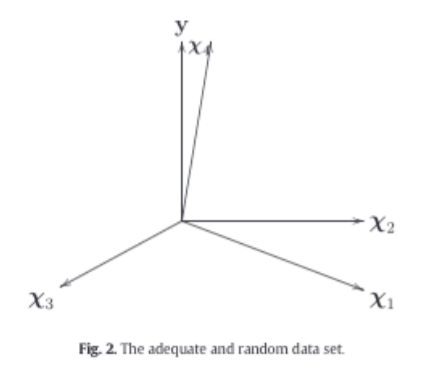
\includegraphics[width=0.7\linewidth]{q4.png}} \\
	\end{minipage}
	\vfill
	\begin{minipage}[h]{0.47\linewidth}
		\center{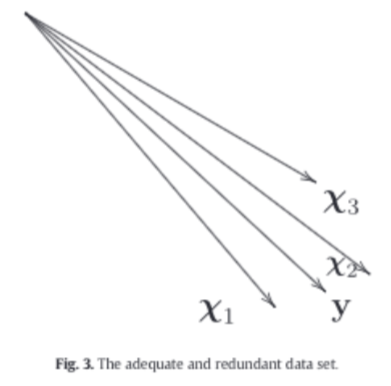
\includegraphics[width=.7\linewidth]{q3.png}}  \\
	\end{minipage}
	\hfill
	\begin{minipage}[h]{0.47\linewidth}
		\center{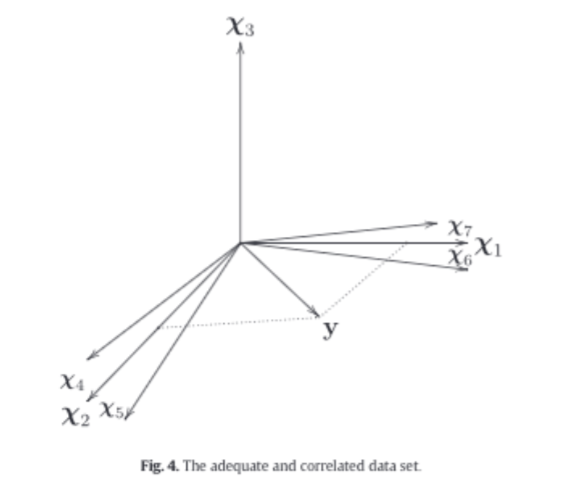
\includegraphics[width=.8\linewidth]{q1.png}} \\
	\end{minipage}
	
\end{figure}

\end{frame}




\begin{frame}{Эксперимент с уровнем шума}


		\center{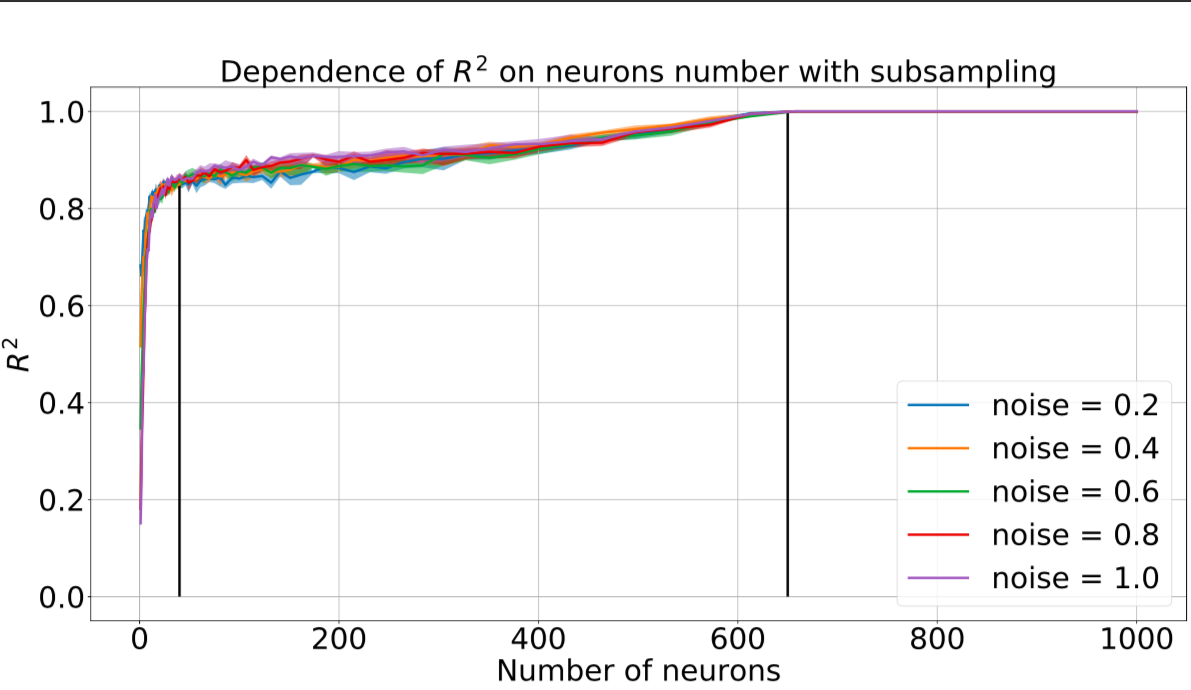
\includegraphics[width=1.\linewidth]{noise_1_w.png} \\ }
			

\end{frame}

\begin{frame}{Эксперимент с уровнем шума}


\center{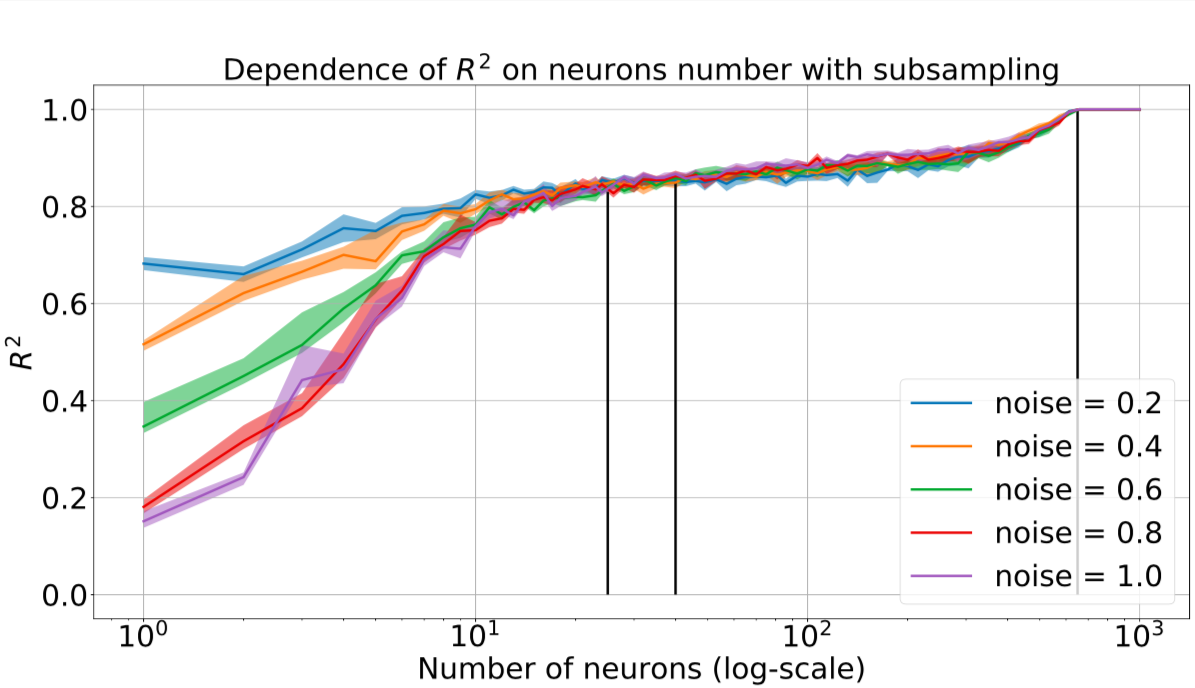
\includegraphics[width=1.\linewidth]{noise_1_.png} \\ }


\end{frame}

\begin{frame}{Эксперимент с количеством кластеров}


\center{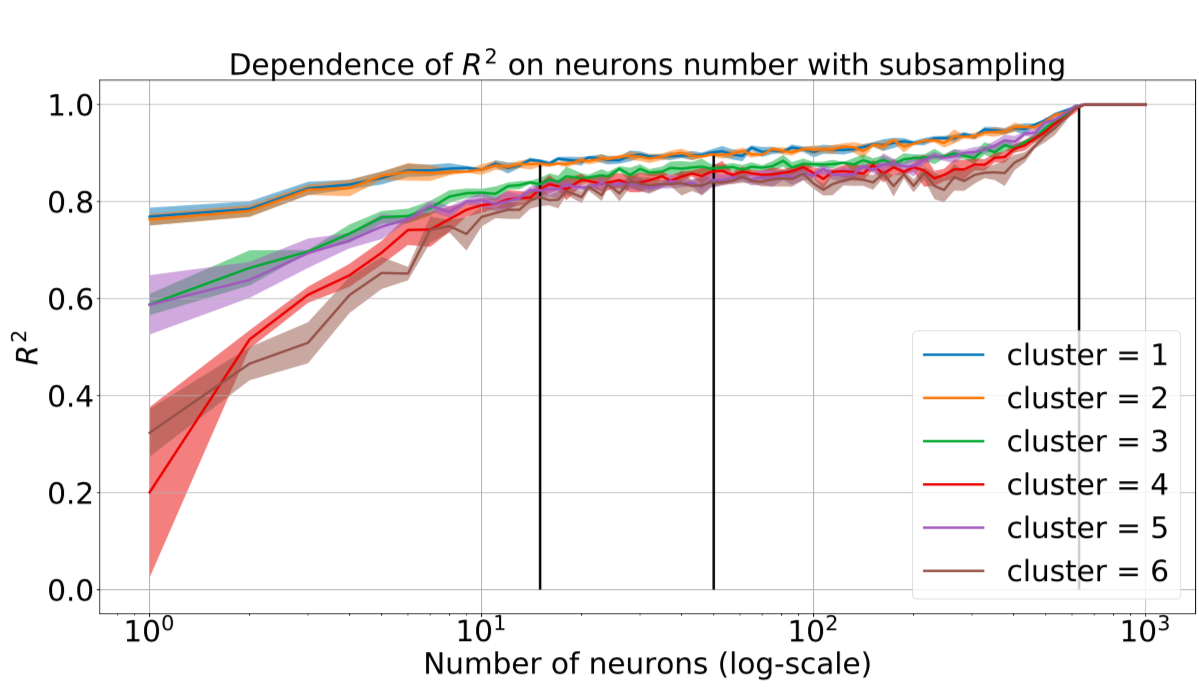
\includegraphics[width=1.\linewidth]{cluster_l2.png} \\ }


\end{frame}

\begin{frame}{Эксперимент с количеством ортогональных признаков}


\center{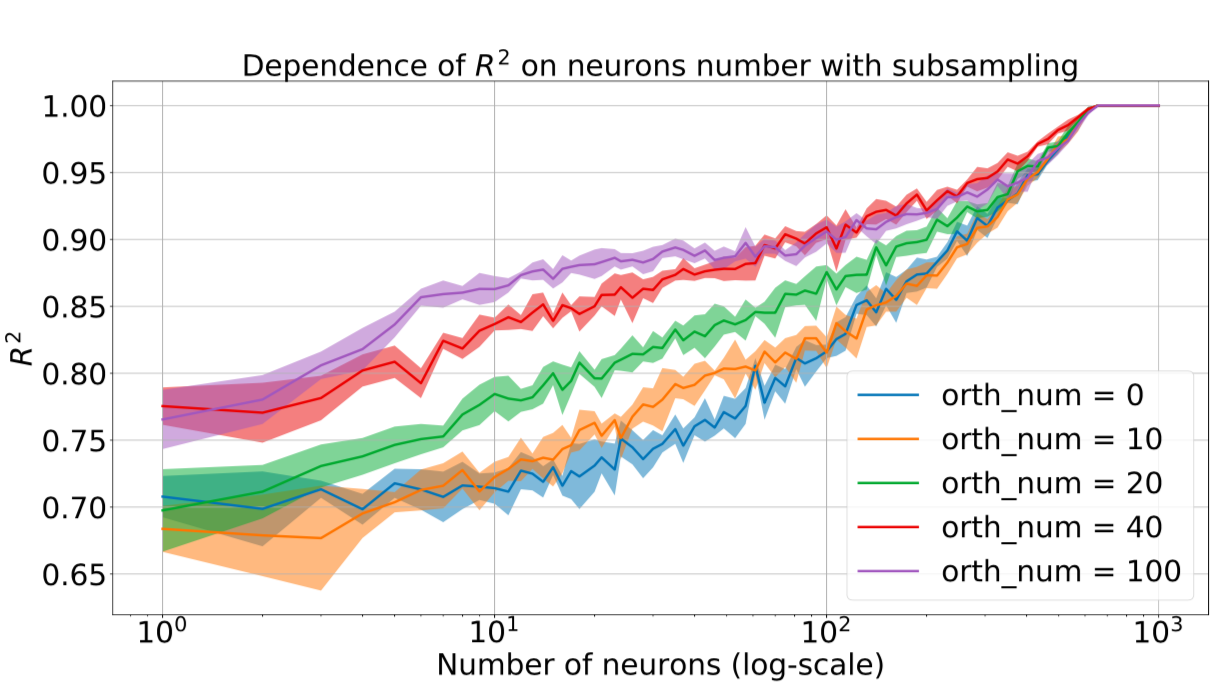
\includegraphics[width=1.\linewidth]{orth1.png} \\ }


\end{frame}
\begin{frame}{Эксперимент с количеством объектов}


\center{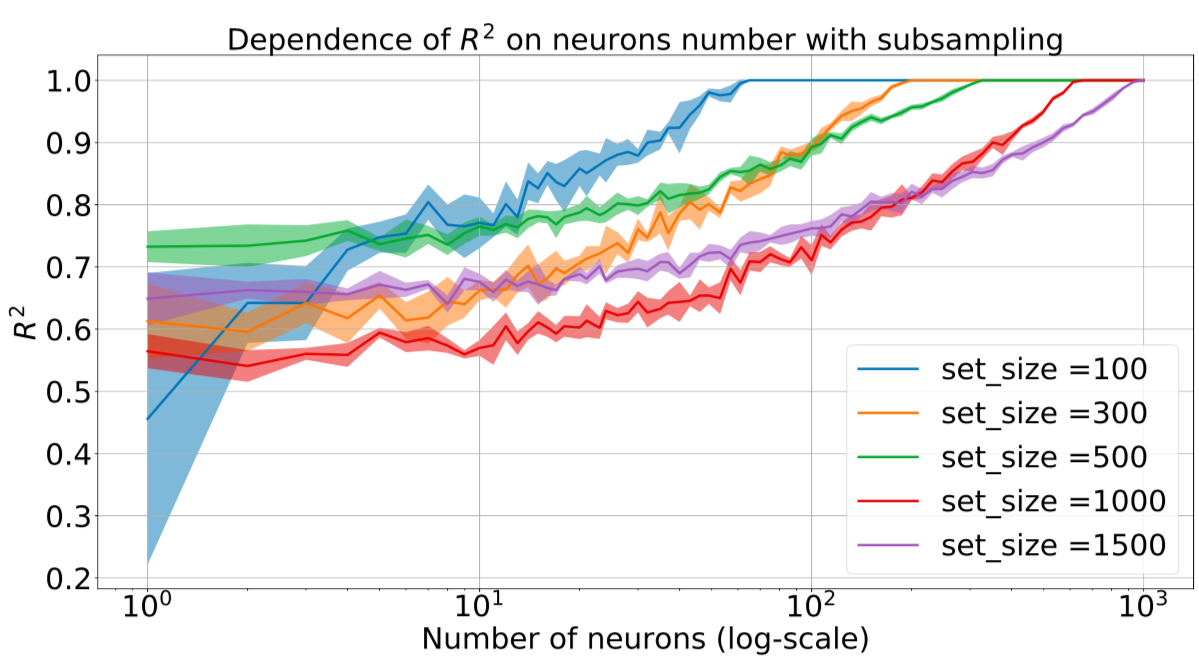
\includegraphics[width=1.\linewidth]{set.png} \\ }


\end{frame}

\begin{frame}{Эксперимент с количеством важных признаков}


\center{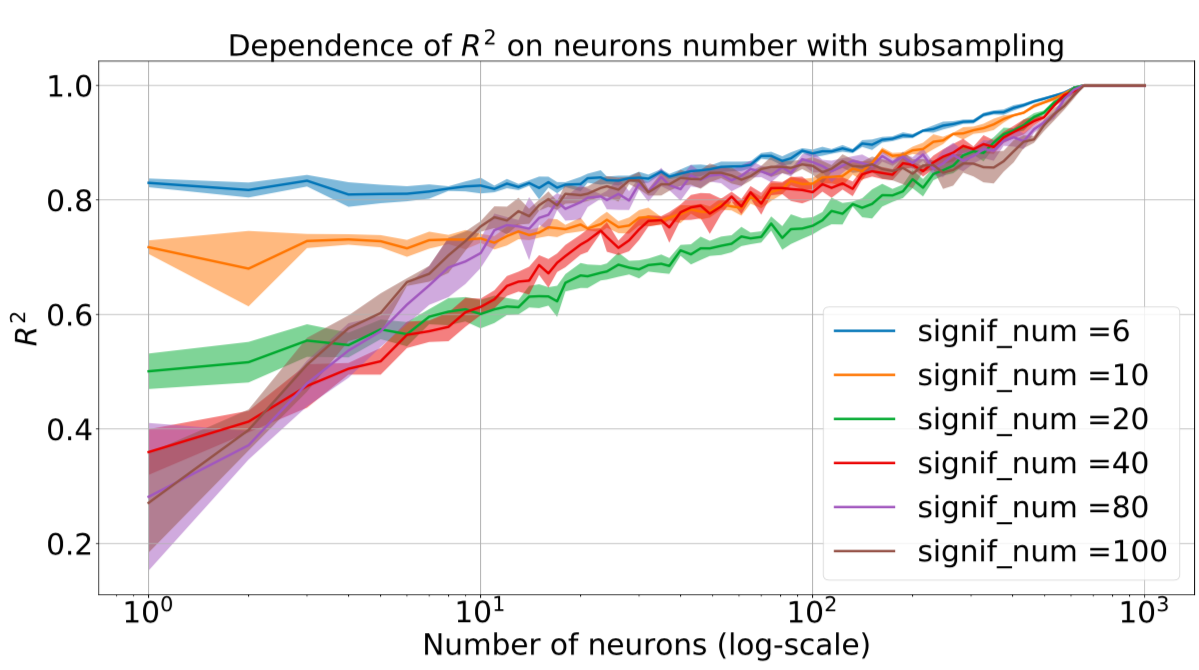
\includegraphics[width=1.\linewidth]{signi.png} \\ }


\end{frame}

%----------------------------------------------------------------------------------------------------------


\end{document} 